\documentclass{article}
\usepackage[left=0.5in,right=0.5in,bottom=0.75in,top=0.75in]{geometry}

% Packages
\usepackage{amsmath}
\usepackage{amssymb}
\usepackage{amsthm}
\usepackage{graphicx}
\graphicspath{{fig/}}
\usepackage{natbib}
\usepackage{hyperref}
\hypersetup{colorlinks=true, citecolor=black, linkcolor=., urlcolor=cyan}
\usepackage[font = small]{caption}
\captionsetup{width=\linewidth}
\usepackage[shortlabels]{enumitem}
\numberwithin{equation}{section}
\usepackage{booktabs}
\usepackage{algpseudocode}
\usepackage{tikz}
\usetikzlibrary{tikzmark}
\usepackage{array} %% required by kableExtra if column_spec
\usepackage[normalem]{ulem}
\usepackage{appendix}

% Theorems and algorithms
\newtheorem{thm}{Theorem}
\algnewcommand\algorithmicswitch{\textbf{switch}}
\algnewcommand\algorithmiccase{\textbf{case}}
\algnewcommand\algorithmicassert{\textbf{then }}
\algnewcommand\Assert[1]{\State \algorithmicassert #1}%
\algnewcommand\Assertif[2]{\State \textbf{if} #1 \algorithmicassert #2}
\algnewcommand\Assertelse[1]{\State \textbf{else} #1}
\algdef{SE}[SWITCH]{Switch}{EndSwitch}[1]{\algorithmicswitch\ #1}{\algorithmicend\ \algorithmicswitch}%
\algdef{SE}[CASE]{Case}{EndCase}[1]{\algorithmiccase\ #1}{\algorithmicend\ \algorithmiccase}%
\algtext*{EndSwitch}%
\algtext*{EndCase}%

% Macros
% Uppercase roman letters
\providecommand{\A}{\mathbf{A}}
\providecommand{\B}{\mathbf{B}}
\providecommand{\C}{\mathbf{C}}
\providecommand{\D}{\mathbf{D}}
\providecommand{\E}{\mathbf{E}}
\providecommand{\F}{\mathbf{F}}
\providecommand{\G}{\mathbf{G}}
\renewcommand{\H}{\mathbf{H}}
\providecommand{\I}{\mathbf{I}}
\providecommand{\J}{\mathbf{J}}
\providecommand{\K}{\mathbf{K}}
\providecommand{\L}{\mathbf{L}}
\providecommand{\M}{\mathbf{M}}
\providecommand{\N}{\mathbf{N}}
\providecommand{\O}{\mathbf{O}}
\renewcommand{\P}{\mathbf{P}}
\providecommand{\Q}{\mathbf{Q}}
\providecommand{\R}{\mathbf{R}}
\renewcommand{\S}{\mathbf{S}}
\providecommand{\T}{\mathbf{T}}
\providecommand{\U}{\mathbf{U}}
\providecommand{\V}{\mathbf{V}}
\providecommand{\W}{\mathbf{W}}
\providecommand{\X}{\mathbf{X}}
\providecommand{\Y}{\mathbf{Y}}
\providecommand{\Z}{\mathbf{Z}}

% Lowercase roman letters (c, d, u, v have to be treated special; see end)
\renewcommand{\a}{\mathbf{a}}
\renewcommand{\b}{\mathbf{b}}
\newcommand{\e}{\mathbf{e}}
\newcommand{\f}{\mathbf{f}}
\newcommand{\g}{\mathbf{g}}
\newcommand{\h}{\mathbf{h}}
\renewcommand{\i}{\mathbf{i}}
\renewcommand{\j}{\mathbf{j}}
\renewcommand{\k}{\mathbf{k}}
\renewcommand{\l}{\mathbf{l}}
\newcommand{\m}{\mathbf{m}}
\newcommand{\n}{\mathbf{n}}
\renewcommand{\o}{\mathbf{o}}
\newcommand{\p}{\mathbf{p}}
\newcommand{\q}{\mathbf{q}}
\renewcommand{\r}{\mathbf{r}}
\newcommand{\s}{\mathbf{s}}
\renewcommand{\t}{\mathbf{t}}
\newcommand{\w}{\mathbf{w}}
\newcommand{\x}{\mathbf{x}}
\newcommand{\y}{\mathbf{y}}
\newcommand{\z}{\mathbf{z}}
\let\origc\c
\DeclareRobustCommand\c{\ifmmode\mathbf{c}\else\expandafter\origc\fi}
\let\origd\d
\DeclareRobustCommand\d{\ifmmode\mathbf{d}\else\expandafter\origd\fi}
\let\origu\u
\DeclareRobustCommand\u{\ifmmode\mathbf{u}\else\expandafter\origu\fi}
\let\origd\v
\DeclareRobustCommand\v{\ifmmode\mathbf{v}\else\expandafter\origv\fi}

%% Roman letters with hats
\providecommand{\fhat}{\hat{f}}
\providecommand{\shat}{\hat{s}}
\providecommand{\yhat}{\hat{y}}
\providecommand{\bfhat}{\hat{\bf f}}
\providecommand{\bshat}{\hat{\mathbf{s}}}
\providecommand{\byhat}{\hat{\mathbf{y}}}

%% Roman letters with subscripts
\providecommand{\rj}{\mathbf{r}_{-j}}
\providecommand{\xj}{\mathbf{x}_{-j}}
\providecommand{\Xj}{\mathbf{X}_{-j}}

%% Roman letters with tildes
\providecommand{\rr}{\tilde{r}}
\providecommand{\xx}{\tilde{x}}
\providecommand{\yy}{\tilde{y}}
\providecommand{\zz}{\tilde{z}}
\providecommand{\brr}{\tilde{\mathbf{r}}}
\providecommand{\bxx}{\tilde{\mathbf{x}}}
\providecommand{\byy}{\tilde{\mathbf{y}}}
\providecommand{\bzz}{\tilde{\mathbf{z}}}
\providecommand{\XX}{\widetilde{\mathbf{X}}}
\providecommand{\WW}{\widetilde{\mathbf{W}}}
\providecommand{\ZZ}{\tilde{\mathbf{Z}}}

%% Script letters
\providecommand{\cA}{\mathcal{A}}
\providecommand{\cB}{\mathcal{B}}
\providecommand{\cC}{\mathcal{C}}
\providecommand{\cD}{\mathcal{D}}
\providecommand{\cE}{\mathcal{E}}
\providecommand{\cF}{\mathcal{F}}
\providecommand{\cG}{\mathcal{G}}
\providecommand{\cH}{\mathcal{H}}
\providecommand{\cI}{\mathcal{I}}
\providecommand{\cM}{\mathcal{M}}
\providecommand{\cN}{\mathcal{N}}
\providecommand{\cR}{\mathcal{R}}
\providecommand{\cS}{\mathcal{S}}
\providecommand{\cT}{\mathcal{T}}
\providecommand{\cU}{\mathcal{U}}
\providecommand{\cV}{\mathcal{V}}
\providecommand{\cW}{\mathcal{W}}
\providecommand{\cX}{\mathcal{X}}
\providecommand{\cY}{\mathcal{Y}}
\providecommand{\cZ}{\mathcal{Z}}

%% Greek letters
\providecommand{\ah}{\hat{\alpha}}
\providecommand{\ba}{\boldsymbol{\alpha}}
\providecommand{\bah}{\hat{\boldsymbol{\alpha}}}
\providecommand{\bb}{\boldsymbol{\beta}}
\providecommand{\bh}{\widehat{\beta}}
\providecommand{\bbh}{\widehat{\boldsymbol{\beta}}}
\providecommand{\bd}{\boldsymbol{\delta}}
\renewcommand{\dh}{\hat{\delta}}
\providecommand{\be}{\boldsymbol{\eta}}
\providecommand{\eh}{\hat{\eta}}
\providecommand{\beh}{\hat{\boldsymbol{\eta}}}
\providecommand{\eps}{\epsilon}
\providecommand{\veps}{\varepsilon}
\providecommand{\bep}{\boldsymbol{\epsilon}}
\providecommand{\bvep}{\boldsymbol{\varepsilon}}
\providecommand{\eph}{\hat{\epsilon}}
\providecommand{\beph}{\hat{\boldsymbol{\epsilon}}}
\providecommand{\gam}{\gamma}
\providecommand{\bg}{\boldsymbol{\gamma}}
\providecommand{\bgh}{\hat{\boldsymbol{\gamma}}}
\providecommand{\bG}{\boldsymbol{\Gamma}}
\providecommand{\gh}{\hat{\gamma}}
\providecommand{\bm}{\boldsymbol{\mu}}
\providecommand{\mh}{\hat{\mu}}
\providecommand{\bmh}{\hat{\boldsymbol{\mu}}}
\providecommand{\lam}{\lambda}
\providecommand{\Lam}{\Lambda}
\providecommand{\bl}{\boldsymbol{\lambda}}
\providecommand{\lh}{\hat{\lambda}}
\providecommand{\bL}{\boldsymbol{\Lambda}}
\providecommand{\bO}{\boldsymbol{\Omega}}
\providecommand{\bp}{\boldsymbol{\pi}}
\providecommand{\ph}{\hat{\pi}}
\providecommand{\bph}{\hat{\boldsymbol{\pi}}}
\providecommand{\bpsi}{\boldsymbol{\psi}}
\providecommand{\sh}{\hat{\sigma}}
\providecommand{\bS}{\boldsymbol{\Sigma}}
\providecommand{\bSh}{\hat{\boldsymbol{\Sigma}}}
\providecommand{\bt}{\boldsymbol{\theta}}
\renewcommand{\th}{\hat{\theta}}
\providecommand{\ts}{\theta^*}
\providecommand{\bth}{\hat{\boldsymbol{\theta}}}
\providecommand{\bts}{\boldsymbol{\theta}^*}
\providecommand{\bT}{\boldsymbol{\Theta}}
\providecommand{\btau}{\boldsymbol{\tau}}
\providecommand{\tauh}{\hat{\tau}}
\providecommand{\btauh}{\hat{\boldsymbol{\tau}}}
\providecommand{\bbj}{\boldsymbol{\beta}_{-j}}
\providecommand{\bbhj}{\widehat{\boldsymbol{\beta}}_{-j}}

%% Greek letters with tildes
\providecommand{\betat}{\widetilde{\beta}}
\providecommand{\bbjt}{\widetilde{\boldsymbol{\beta}}_{-j}}
\providecommand{\bbt}{\widetilde{\boldsymbol{\beta}}}
\providecommand{\etat}{\tilde{\eta}}
\providecommand{\bet}{\widetilde{\boldsymbol{\eta}}}
\providecommand{\lamt}{\tilde{\lambda}}
\providecommand{\mt}{\tilde{\mu}}
\providecommand{\bmt}{\tilde{\boldsymbol{\mu}}}
\providecommand{\nut}{\tilde{\nu}}
\providecommand{\thetat}{\tilde{\theta}}
\providecommand{\btt}{\tilde{\boldsymbol{\theta}}}

%% Operators
\renewcommand{\Pr}{\mathbb{P}}
\providecommand{\pr}{\textrm{Pr}}
\providecommand{\Ex}{\mathbb{E}}
\providecommand{\ex}{\textrm{E}}
\providecommand{\exh}{\widehat{\textrm{E}}}
\providecommand{\Var}{\mathbb{V}}
\providecommand{\var}{\textrm{Var}}
\providecommand{\varh}{\widehat{\textrm{Var}}}
\providecommand{\cov}{\textrm{Cov}}
\providecommand{\cor}{\textrm{Cor}}
\providecommand{\trace}{\textrm{tr}}
\providecommand{\rank}{\textrm{rank}}
\providecommand{\Norm}{\textrm{N}}
\providecommand{\Gmma}{\textrm{Gamma}}
\providecommand{\Beta}{\textrm{Beta}}
\providecommand{\Pois}{\textrm{Pois}}
\providecommand{\NBin}{\textrm{NegBin}}
\providecommand{\Unif}{\textrm{Unif}}
\providecommand{\Binom}{\textrm{Binom}}
\providecommand{\Bern}{\textrm{Bern}}
\providecommand{\Weib}{\textrm{Weibull}}
\providecommand{\Scx}{\textrm{Scaled-}\chi^2}
\providecommand{\Wish}{\textrm{Wishart}}
\providecommand{\Multinom}{\textrm{Multinom}}
\providecommand{\Dirch}{\textrm{Dir}}
\providecommand{\Exp}{\textrm{Exp}}
\providecommand{\diag}{\textrm{diag}}
\providecommand{\Tr}{^{\scriptscriptstyle\top}}

%% Statistical
\renewcommand{\l}{\ell}
\providecommand{\inP}{\overset{\textrm{P}}{\longrightarrow}}
\providecommand{\inAS}{\overset{\textrm{as\,}}{\longrightarrow}}
\providecommand{\inD}{\overset{\textrm{d}}{\longrightarrow}}
\providecommand{\inQM}{\overset{\textrm{qm\,}}{\longrightarrow}}
\providecommand{\adist}{\overset{\text{.}}{\sim}}
\providecommand{\AIC}{\textrm{AIC}}
\providecommand{\BIC}{\textrm{BIC}}
\providecommand{\CI}{\textrm{CI}}
\providecommand{\CV}{\textrm{CV}}
\providecommand{\FWER}{\textrm{FWER}}
\providecommand{\FDR}{\textrm{FDR}}
\providecommand{\FDRh}{\widehat{\textrm{FDR}}}
\providecommand{\fdr}{\textrm{fdr}}
\providecommand{\fdrh}{\widehat{\textrm{fdr}}}
\providecommand{\Fdr}{\textrm{Fdr}}
\providecommand{\Fdrh}{\widehat{\textrm{Fdr}}}
\providecommand{\GCV}{\textrm{GCV}}
\providecommand{\KL}{\textrm{KL}}
\providecommand{\LR}{\textrm{LR}}
\providecommand{\ME}{\textrm{ME}}
\providecommand{\MLE}{\textrm{MLE}}
\providecommand{\MSE}{\textrm{MSE}}
\providecommand{\MSPE}{\textrm{MSPE}}
\providecommand{\OLS}{\textrm{OLS}}
\providecommand{\PE}{\textrm{PE}}
\providecommand{\RSS}{\textrm{RSS}}
\providecommand{\SNR}{\textrm{SNR}}
\providecommand{\SE}{\textrm{SE}}
\providecommand{\SD}{\textrm{SD}}
\providecommand{\OR}{\textrm{OR}}
\providecommand{\RR}{\textrm{RR}}
\providecommand{\df}{\textrm{df}}
\providecommand{\odds}{\textrm{odds}}
\providecommand{\loglik}{\textrm{loglik}}
\providecommand{\logit}{\textrm{logit}}
\providecommand{\const}{\textrm{constant}}

% Fisher/observed information
\usepackage[scr=boondox]{mathalpha}
\providecommand{\oI}{\boldsymbol{\mathcal{I}}}
\providecommand{\oV}{\boldsymbol{\mathcal{V}}}

\makeatletter
\@ifpackagelater{mathalpha}{2021/01/01}{%
\providecommand{\fI}{\mathbfscr{I}}
\providecommand{\fV}{\mathbfscr{V}}
}{%
\providecommand{\fI}{\mathbscr{I}}
\providecommand{\fV}{\mathbscr{V}}
}
\makeatother

% Independence
\providecommand{\iid}{\overset{\text{iid}}{\sim}}
\providecommand{\ind}{\perp\!\!\!\perp}
\providecommand{\IID}{\overset{\scriptscriptstyle \ind}{\sim}}

%% Mathematical
\providecommand{\one}{\mathbf{1}}
\providecommand{\zero}{\mathbf{0}}
\providecommand{\intii}{\int_{-\infty}^{\infty}}
\providecommand{\real}{\mathbb{R}}
%%\providecommand{\Real}{\mathds{R}} %% Requires dsfonts
\providecommand{\dl}{d_-}
\providecommand{\dr}{d_+}
\providecommand{\sign}{\textrm{sign}}
\providecommand{\given}{\,\vert\,}
\providecommand{\abs}[1]{\left\lvert#1\right\rvert}
\providecommand{\sabs}[1]{\lvert#1\rvert}
\providecommand{\norm}[1]{\lVert#1\rVert}
\providecommand{\bignorm}[1]{\left\lVert#1\right\rVert}
\providecommand{\gl}{\prec}
\providecommand{\gle}{\preceq}
\providecommand{\gg}{\succ}
\providecommand{\gge}{\succeq}
\DeclareMathOperator*{\argmin}{\arg\min}
\DeclareMathOperator*{\argmax}{\arg\max}
\providecommand{\pf}[2]{\frac{\partial #1}{\partial #2}}

%% Equations
\providecommand{\al}[2]{\begin{align}\label{#1}#2\end{align}}
\providecommand{\as}[1]{\begin{align*}#1\end{align*}}
\providecommand{\als}[2]{\begin{align}\label{#1}\begin{split}#2\end{split}\end{align}}
\providecommand{\tcirc}[1]{\raisebox{.5pt}{\textcircled{\raisebox{-.9pt} {#1}}}}

% Other
\providecommand{\note}[1]{\textcolor{red}{#1}}
\providecommand{\MAF}{\textrm{MAF}}


% Notes to each other
\newcommand{\pb}[1]{\textcolor{red}{#1}}
\newcommand{\logan}[1]{\textcolor{blue}{#1}}

% Define abstract environment
\renewcommand{\abstract}[1]{
 \centerline{
 \begin{minipage}{0.7\linewidth}
 \hrule
 \vskip 0.1in
  \begin{center}
    {\bf Abstract}
  \end{center}
  #1
 \vskip 0.1in
 \hrule
 \end{minipage}}
 \vskip 0.3in}

% Title/author/date
\title{Lasso confidence intervals: Another look at the bootstrap}
\author{
  Logan Harris\\Department of Biostatistics\\University of Iowa
  \and
  Patrick Breheny\\Department of Biostatistics\\University of Iowa
}
\date{\today}


\begin{document}

\maketitle

\abstract{Abstract goes here.}

\section{Introduction}

The prevailing opinion is that the traditional use of bootstrapping to produce confidence intervals for penalized regression is suboptimal due to the inherent behavior of estimates produced by penalization.

Specifically, we see two potential problems that arise when proposing to use bootstrapping for penalized regression, we will refer to these obstacles as,

\begin{enumerate}
\item the Bias Tradeoff, and \logan{Better term?}
\item the Epsilon Conundrum.
\end{enumerate}

The Bias Tradeoff refers to the inherent bias introduced by penalization in order to be able to fit oversaturated models. This penalization leads to coverages much higher than nominal coverage rates for coefficients with true values at or very near zero and leads to much lower coverage when coefficients are non-zero. We argue that coverage in the traditional sense is too ridged of a paradigm to apply to penalized regression inference. Instead, we offer a different perspective and argue that the impact that penalization induced bias has is an inherent feature of penalized regression rather than a flaw. Since high dimensional problems often necessitate such an alternate approach, we offer guidance on how to interpret the confidence intervals for lasso as presented in this paper. Additionally, we compare the proposed method to two other inferential methods which take a different perspective.

The second problem, the Epsilon Conundrum, is also related to the shrinkage but arises as an arguably more disturbing manifestation: confidence intervals of length zero or, more often, with a single endpoint that is exactly zero. Some penalized regression methods, particularly the lasso, often result in a sparse solution. If using a traditional quantile based bootstrap confidence interval, this will lead to an interval of [0,0] if a given variable is rarely or never included in the active set. As the dimensionality of the problem grows, this becomes an increasing occurrence leading to a large majority of intervals possessing a length of zero. When the true value of the coefficient is 0, the interval at least contains the truth. However, this issue is particularly troublesome when one considers what happens when the true value is not precisely zero, as is likely the case in most reasonable scenarios. By just shifting the true value by $\eps$, an immediate drop in coverage would occur, hence the name: the Epsilon Conundrum.

The later of these two problems is addressed in our novel approach to producing bootstrap based confidence intervals for the lasso.

\section{Inferential Paradigm}

The method to be proposed falls into a bit of a grey area that isn't well encapsulated by common interential scopes such as "marginal", "conditional", or "joint". To that end, we breifly describe a different perspective here which we call \textit{Order Inference}.

The idea of \textit{Order Inference} focuses on the variable space which inferential methods are conducted. Specifcally, we will let order referece the relation of the current variable under consideration, $\x_i$, to the other variables, $\x_j$, where $j \neq i$ as well as their relation to the outcome variable $\y$. To visualize the concept of \textit{Order Inference}, we will provide a simple example using multiple linear regression.

\textbf{Zeroth Order} ($O_z$): Here, no consideration is given to $\x_j$. All inference for $\beta_i$ is done based on the residuals from $\hat{y}$ as a projection onto the column space of $X_i$.

\textbf{First Order} ($O_1$): In this paradigm, this is the most difficult to capture since it could take a few forms. The way this occurs is by projecting $\y$ first onto the columns space of $\X_j$ then the residuals $\r_j$ onto the column space of $\X_i$. How the first projection occurs is where alternatives forms into play. A literal translation would involve p two-step regressions. An alternate form that is more akin to the approach to be proposed requires one joint regression, calculation of partial residuals $\r_{-i}$ then projecting $\r_{-i}$ onto the column space of $\x_i$.

\textbf{Second Order} ($O_2$): With $n \gg p$ and $\epsilon \sim N(0, \sigma^2)$, this is the traditional analysis most would run: perform joint inference with residuals from $\hat{y}$ as a projection onto the column space of $\boldsymbol{X}$.

\section{Lasso Bootstrap Confidence Intervals}

As with other penalized regression models, the lasso can be formulated as a Bayesian regression model by setting an appropriate prior. For the lasso, this prior is a Laplace, also called double-exponential, distribution:

\as{\p(\bb) = \prod_{j = 1}^{p} \frac{\gamma}{2}\exp(-\gamma \abs{\beta_j}), \gamma > 0}

With this prior, the lasso estimate $\bbh(\lam)$ is the posterior mode of $\bb$ when $\lam = \gamma \frac{\sigma^2}{n}$.

We propose leveraging this relationship to build confidence intervals for $\bb$. Specifically, we propose the following process for given values of $\lam$, $\sigma^2$, and significance level, $\l$:

\begin{enumerate}
\item Obtain a bootstrap sample of $\X$ and $\y$
\item For each $\beta_j$:
	\begin{enumerate}
	\item Obtain the first-order, $O_1$, posterior for $\beta_j$
	\item Draw r randomly selected quantiles and save
	\end{enumerate}
\item Repeat m times
\item For each $\beta_j$, combine the r*m samples and compute the quantiles for $p_L = (.5 - \l/2)$ and $p_U = (.5 + \l/2)$
\end{enumerate}

\section{Details}

In this section, we describe the details of each of the steps outlined above along with other important considerations.

\subsection{Bootstrap Sampling}

There are various ways to perform a single iteration of a bootstrap, among them are the pairs bootstrap and the residual bootstrap. For high dimensional problems in general, the pairs bootstrap is attractive. First, it makes the fewest assumptions compared to other methods. Specifically, the only assumption made for the pairs bootstrap is that the original pairs were randomly sampled from some distribution $F$, where $F$ is a distribution on (p + 1)-dimensional vectors (Efron, Tibshirani). Additionally, the pairs bootstrap is simple to perform. Finally, and perhaps most importantly, it treats $\X$ as random which is almost surely the case in high dimensional settings. For this reason, we will solely focus on and use the pairs bootstrap in our proposed procedure.

\subsection{Obtaining Intervals}

\subsubsection{Computing the \texorpdfstring{$O_1$}{first order} posterior for \texorpdfstring{$\beta_j$}{betaj}}

Unfortunately, a Normal likelihood and Laplace prior are not conjugate and in general, the absolute value in the exponent of the Laplace makes many common manipulations for the posterior more difficult. Luckily, however, the marginal posterior can be shown to be a mixture of a right and left truncated normal where the truncation occurs at zero for right and left tails respectively. To obtain a $O_1$ posterior, we use the partial residuals, $\r_{-j}$, in the likelihood. This is natural due to the common CD algorithms used to arrive at lasso estimates. In the steps that follow, we will assume that $\X$ has been standardized s.t. $\x_j^T\x_j = n$. For $\beta_j$,

\as{
L(\beta_j | \r_{-j}) &= (\sigma \sqrt{2\pi})^{-n} \exp(-\frac{1}{2\sigma^2} (n\beta_j^2 - 2\x_{j}^{T}\r_{-j}\beta_j + \r_{-j}^{T}\r_{-j})) \\
&\propto \exp(-\frac{n}{2\sigma^2} (\beta_j^2 - 2z_j\beta_j)), \text{ where } z_{j} = \frac{1}{n} \x_{j}^{T}\r_{-j} \\
\Rightarrow P(\beta_j | \r_{-j}) &\propto \exp(-\frac{n}{2\sigma^2} (\beta_j^2 - 2z_{j}\beta_j)) \frac{n \lambda}{2 \sigma^2} \exp(-\frac{n \lambda} {\sigma^2} \abs{\beta_j}) \\
&\propto \exp(-\frac{n}{2\sigma^2} (\beta_j^2 - 2 z_j\beta_j +  2 \lambda \abs{\beta_j})) \\
&= \exp(-\frac{n}{2\sigma^2} (\beta_j^2 - 2(z_j\beta_j - \lambda \abs{\beta_j}))) \\
&=
\begin{cases}
\exp(-\frac{n}{2\sigma^2} (\beta_j^2 - 2(z_j + \lambda)\beta_j)), \text{ if } \beta_j < 0, \\
\exp(-\frac{n}{2\sigma^2} (\beta_j^2 - 2(z_j - \lambda)\beta_j )), \text{ if } \beta_j \geq 0 \\
\end{cases} \\
&\propto
\begin{cases}
C_{-} \exp(-\frac{n}{2\sigma^2} (\beta_j - (z_j + \lambda))^2), \text{ if } \beta_j < 0, \\
C_{+} \exp(-\frac{n}{2\sigma^2} (\beta_j - (z_j - \lambda))^2), \text{ if } \beta_j \geq 0 \\
\end{cases}
}

Where, $C_{-} = \exp(\frac{z_j \lambda n}{\sigma^2})$ and $C_{+} = \exp(-\frac{z_j \lambda n}{\sigma^2})$.

Ignoring the truncation for a moment and focusing on the kernels individually, we can see that the two distributions above are what we would expect from the lasso solution, having a mean $z_j + \lambda$ and $z_j - \lambda$ respectively and a variance of $\frac{\sigma^2}{n}$. That said, due to the truncation, the variance of the posterior is less than or equal to this (plot the $O_1$ posterior and this should become immediately clear). Furthermore, a mapping allows tail probabilities from the posterior to be translated to probabilities onto corresponding known normal distributions ($\N(0, z_j \pm \lambda, \frac{\sigma^2}{n})$). For this translation, we need two pieces of information:

\begin{enumerate}
\item The non-truncated probability in each of the two normals to transformed on to, denoted $Pr_{-}$ and $Pr_{+}$ respectively.
\item The probability in each of the tails of the posterior, denoted $Post_{-}$ and $Post_{+}$ respectively.
\end{enumerate}

(1) is trivial to compute with any statistical software. Similarly, (2) is conceptually simple, although care must be taken to avoid the pitfall of numerical instability introduced as n increases.

To reduce the number of computational steps, one may note that:

\as{
P(\beta_j | \r_{-j})  & \propto
\begin{cases}
C_{-} Pr_{-}, \text{ if } \beta_j < 0, \\
C_{+} Pr_{+}, \text{ if } \beta_j \geq 0 \\
\end{cases}
}

Which implies that $Post_- = \frac{C_{-} Pr_{-}}{C_{-} Pr_{-} + C_{+} Pr_{+}}$ and similarly for $Post_+$. However, to avoid numerical instability, or at least handle it properly when it is unavoidable we need to work on the $\log$ scale. This works well for most of the problem, but computation of $Post_-$ and $Post_+$ need something a bit more since, for example, $\log(Post_-) = \log(C{-}Pr_{-}) - \log(C_{-} Pr_{-} + C_{+} Pr_{+})$. That is, the denominator still must be computed then the $\log$ taken which does not allow operating on the $\log$ scale to fully address potential instability. Instead, $\log(Post_-)$ can be computed with $\log(C_-Pr_-) -  \log(C_+Pr_+) - \log(1 + \exp(\log(C_-Pr_-) -  \log(C_+Pr_+)))$. This still doesn't completely address the issue, however, if $exp(\log(C_-Pr_-) -  \log(C_+Pr_+))$ is infinite then $C_-Pr_- >> C_+Pr_+$ and $\log(Post_-) \approx 0$.

With these values, we can compute quantiles by mapping the corresponding probabilities $p$ for the posterior onto the probabilities $p^*$ for the corresponding normals. Which normal the quantiles of interest ultimately come from is determined based on the values in (2). For example, if $Post_{+} = 0.98$ and $p = 0.1$ the $p$ would be mapped onto the positive normal. As one more example, say $Post_{+} = 0.4$ and $p = 0.5$, then $p$ would be mapped onto the lower normal. The transformation to map a given probability from the posterior depends on which tail the quantile resides in on the posterior (equivalently which normal it is being mapped to, the positive or negative). This map is simply:

\as{
p^* &= p \times (Pr_{\pm} / Post_{\pm}) \\
}

Once this respective probabilities are mapped, one can simply use the inverse of the normal CDFs that the probabilities were mapped to. That being said, there is a nuance worth pointing out. When transforming the probabilities, the step to determine which tail the respective quantile comes from occurs first. With this, the probability should be adjusted so that it refers to the probability between the quantile of interest and the respective tail. After this, then the transformation can be applied.

\logan{Need a better term for the two halves than tail....}

This solution corresponds to a particular value of $\lam$ and $\hat{\sigma}^2$. The only thing prohibitive to producing intervals for the entire lasso path is computational resources since the bootstrap is already computationally expensive. That brings our decision down to producing an estimate for $\sigma^2$. Our recommendation is to first use cross validation (CV) once to produce an estimate. However, note that producing an estimate in this manner implicitly depends on $\lam$, so new estimates for $\sigma^2$ should be obtained for each value of $\lam$.

Our recommendation is to use CV to select $\lam$ and produce an estimate for $\sigma^2$ and produce bootstrap confidence intervals corresponding to these values to report.

All together this leads to the following steps to perform the bootstrap (presented on original scale for compactness):

\begin{enumerate}
\item Perform CV using the original data to select $\lam$ and estimate $\hat{\sigma}^2(\lam)$
\item For i $\in \lbrace 1 \ldots m \rbrace$:
\begin{enumerate}
\item Obtain a pairs bootstrap sample, $\X^*$ and $\y^*$
\item Fit lasso with $\X^*$ and $\y^*$
\item For j $\in \lbrace 1, \ldots, p \rbrace$:
	\begin{enumerate}
	\item Obtain the partial residuals, $r_{-j}$ and compute $z_j$
	\item Compute $Pr_{-}$ = $\Phi(0, z_j + \lam, \frac{\sh^2}{n})$ and $Pr_{+}$ = $1 - \Phi(0, z_j - \lam, \frac{\sh^2}{n})$
	\item Compute $Post_-$ and $Post_+$
	\item For $r$ $\in \lbrace 1, \ldots, R \rbrace$:
	\begin{algorithmic}
		\If {$p_r \leq Post_{-}$}
			\State $q_r = \Phi^{-1}(p_r(Pr_{-} / Post_{-}), z_j + \lam, \frac{\sh^2}{n})$
		\Else
			\State $q_r = \Phi^{-1}(1 - (1 - p_r)*(Pr_{+} / Post_{+}), z_j - \lam, \frac{\sh^2}{n})$
		\EndIf
	\end{algorithmic}
	\item Save $\q$
	\end{enumerate}
\end{enumerate}
\item For each $\beta_j$, combine the $r*m$ samples and compute the quantiles for $p_L = (.5 - \l/2)$ and $p_U = (.5 + \l/2)$ to produce a final confidence interval estimate
\end{enumerate}

\section{Simulation Studies}

\subsection{Overall vs. per-feature coverage}

\includegraphics[width=\linewidth]{overall_v_feature.pdf}

\subsection{Across \texorpdfstring{$\lambda$}{lambda} Performance}
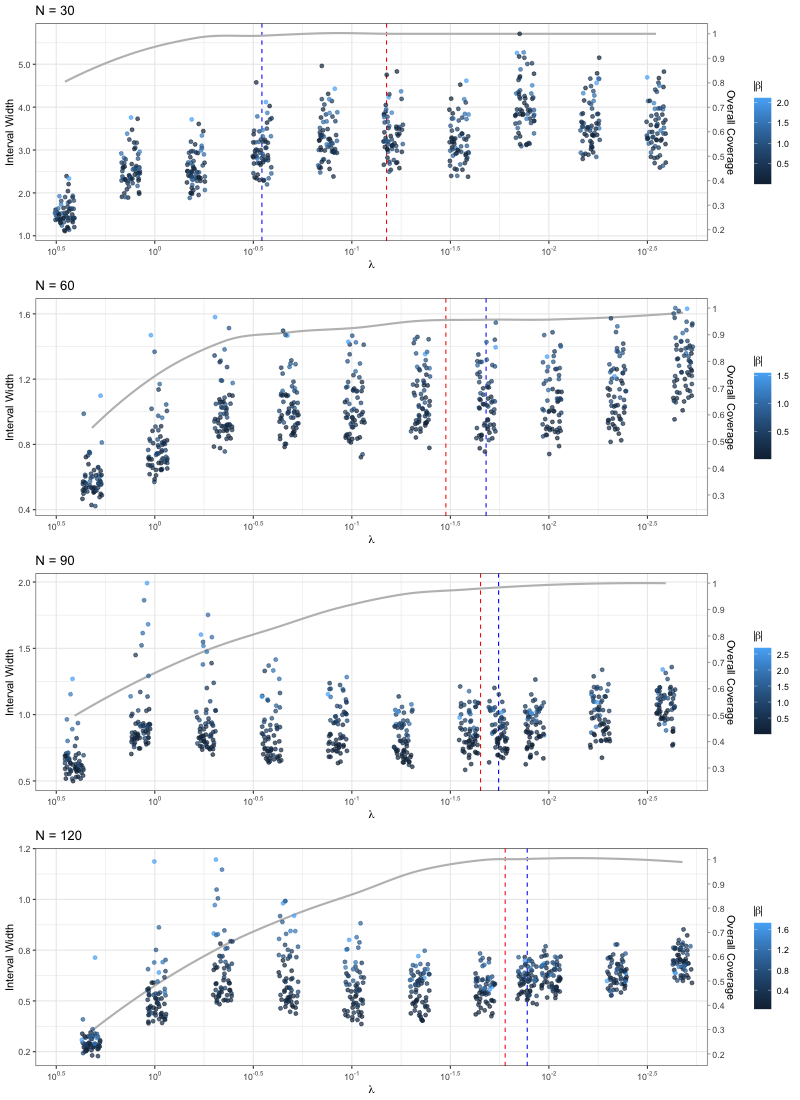
\includegraphics[width=\linewidth]{across_lambda_coverage_laplace.pdf}


\subsection{Distribution of Beta}

\includegraphics[width=\linewidth]{distribution_of_beta.pdf}

\subsection{Epsilon Conundrum (Comparison to Traditional Quantile Bootstrap)}

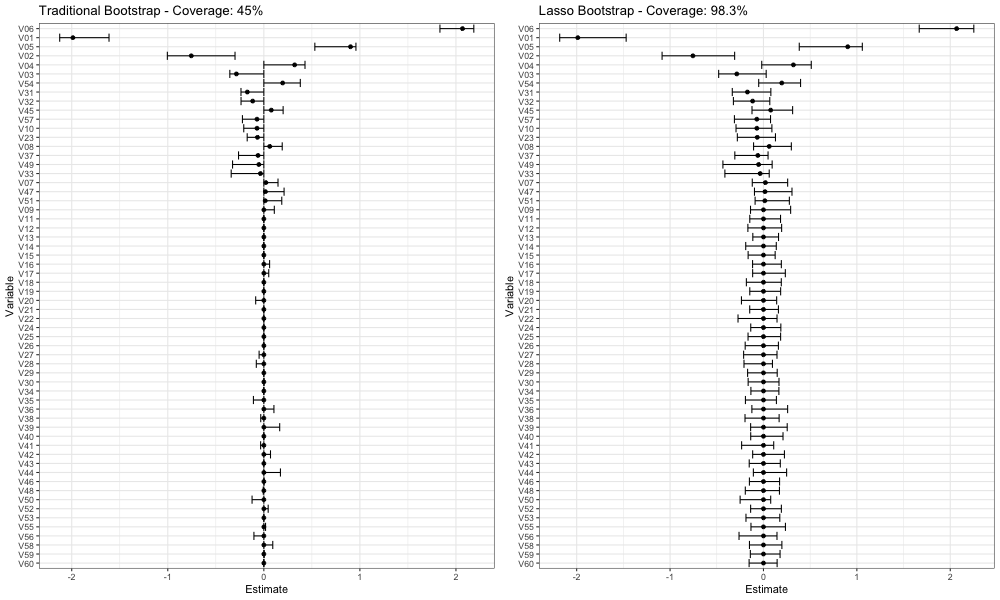
\includegraphics[width=\linewidth]{method_comparison_traditional.pdf}

\subsection{Correlated Features (Comparison to Ridge)}

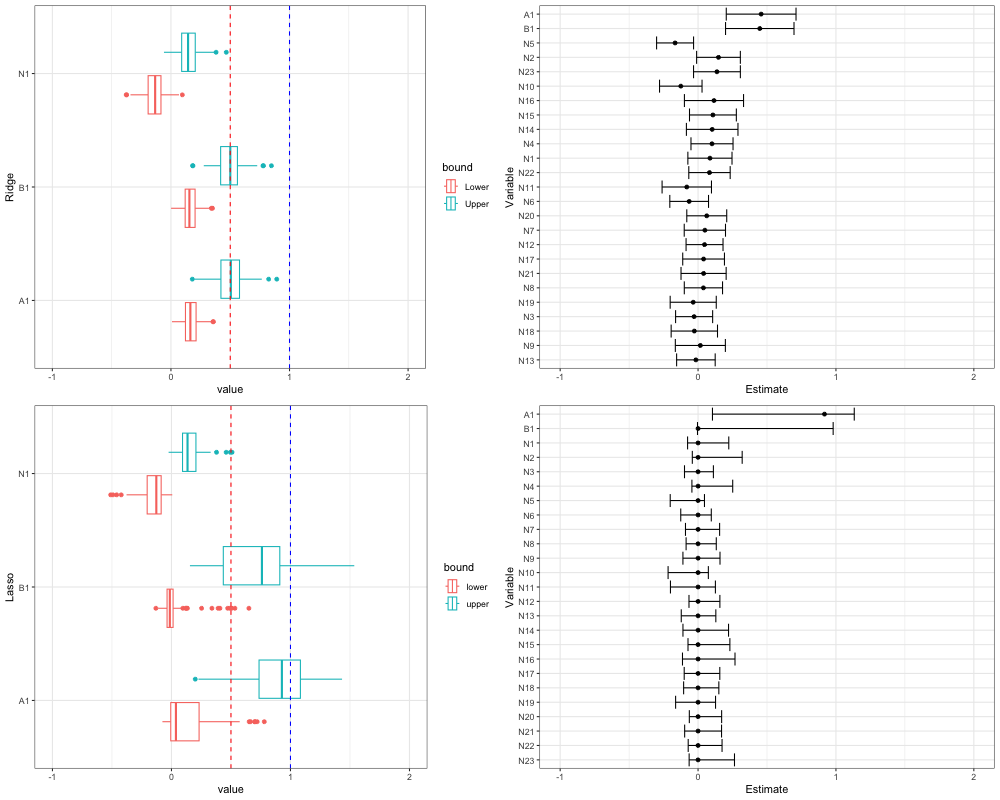
\includegraphics[width=\linewidth]{method_comparison_highcorr_100.pdf}

\subsection{Comparison to Other Methods}

\begin{enumerate}
\item Selective inference
\begin{enumerate}
\item Does not work for $p > n$ case
\item Only produced CI for variables in active set
\item Seems cumbersome and unstable as implemented
\item Unclear recommended selection of $\lam$
\item Non-finite endpoints not uncommon
\end{enumerate}
\item{Bootstrap Lasso Projection}
\end{enumerate}

\subsection{Single Example}

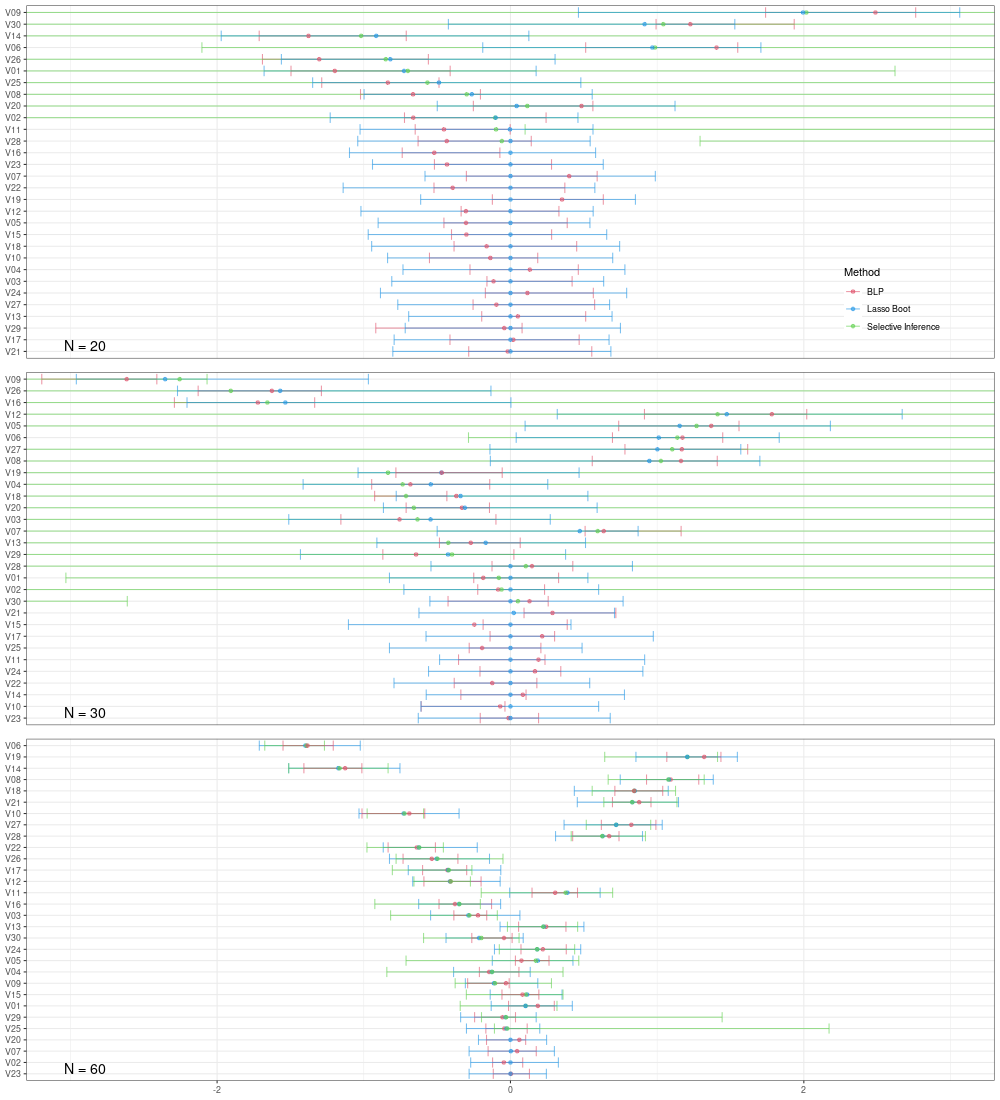
\includegraphics[width=\linewidth]{method_comparison_laplace.pdf}

\subsection{Comparison Similation}

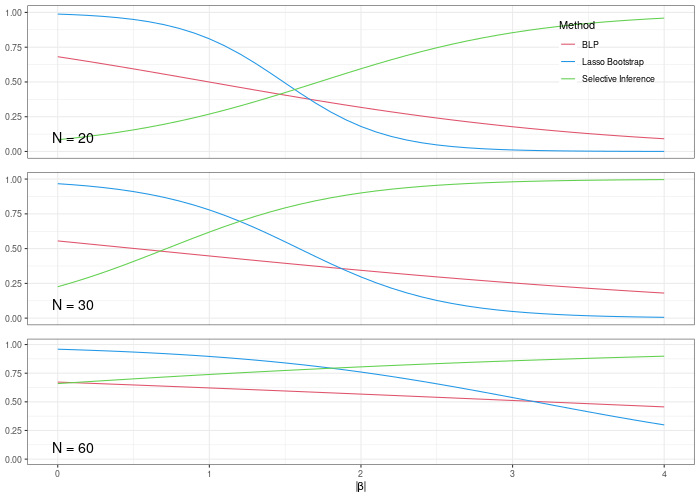
\includegraphics[width=\linewidth]{method_comparison_laplace_100.pdf}

\includegraphics[width=\linewidth]{method_comparison_laplace_100_other.pdf}

\section{Real data}
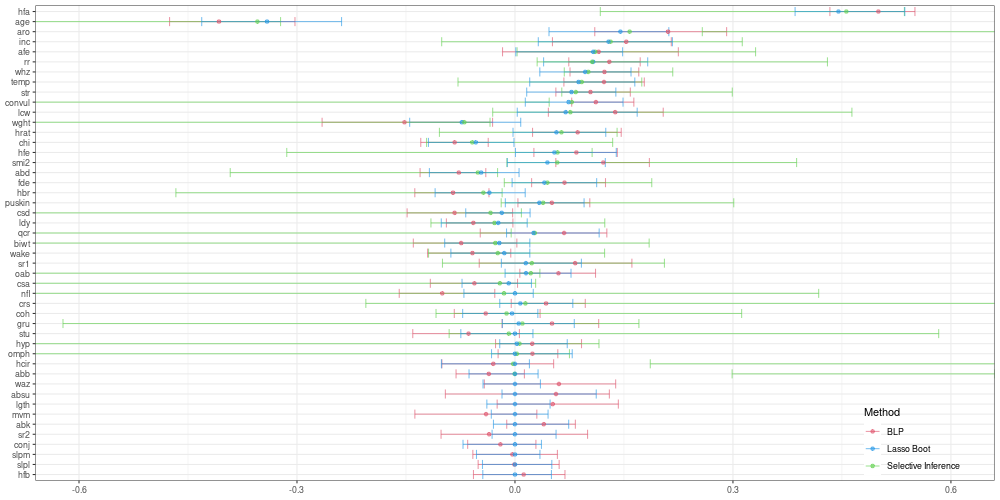
\includegraphics[width=\linewidth]{method_comparison_whoari.pdf}

\section{Limitations}

\subsection{Space Requirements}

As implimented, this method takes a numeric matrix size $Br \times p$. With $B = 100, r = 10$, the sample matrix gets too large enough to cause memory concerns even when $p$ is on the order of $1e5$. For many datasets, this is likely not of concern. however, given that lasso is often used for datasets where $p$ is large, it is clearly not an edge case where $p$ exceeds the order of $1e5$. One could reduce the number size of the same matrix by reducing the number of draws, i.e. let $r = 1$, but this is unstaisfactoy and produces little additional leeway for what seems like a unnacceptable sacrifice. What we propose instead is using incremental quantile estimation as introduced by \cite{Tierney1983}. Although not currently part of the method in \texttt{ncvreg} at the time of this publication, this is an active area of implimentation. Incremental quantile estimation is an ongoing area of research, espeically in feilds like computer networking.

One concern here is that the additional approximation in incremental quantile estimation could result in larger errors, however, it is our belief that these errors will be small in relation to the approximations already a part of the method. Addiitonally, we believe that the errors introduced by incremental quantile estimation will quickly be offset by the ability to have obtained orders of magnitude more draws.

This of course opens up the large question of what method to use for incremental quantile estimation.

We are currently working on implimenting and assessing using the method introduced by \cite{Tierney1983}, but this is an area of ongoing interest for us.

Luckily, as far as problems go, this is a relatively benign use case. The primary obsticle that a method needs to be able to address is adhering to space requirements. Ideally, the storage space required should not grow with the number of draws or should at least grow at a much slower rate than the number of draws (i.e. no faster than $\log(\# of draws)$). In fact, per quantile tracked, the method presented by Tierney only requries 6 direct access storage points. As \cite{Tierney1983} notes, his method only has the requirement that F has "a bounded derivative that is continuous at $\xi$", where $\xi$ is the tracked quantile. The only point at which this could be violated for the distributions we are tracking would be if $\xi = 0$, since the derivative is not necessarily continuous at this point. However, since the distribution itself is continous at 0, $\xi = 0$ w.p. 0.

One drawback of using the method as introduced by Tierney is that is only addresses tracking of a single quantile at a time. Recent research has focused on joint quantile tracking. Future exploration into how such methods perform would undoubtably add robustness, however, given the use case here of tracking two quantiles in seperate tails, we accept this limitation with caution.

\section{Discussion}

\section{Conclusions}

\section*{Acknowledgments}

\section*{Appendix}


\bibliographystyle{ims-nourl}
\bibliography{lasso-boot}

\newpage

\section*{Supplemental material}
\beginsupplement

\section{Sampling from the Full Conditional Posterior}\label{Sup:A}

\logan{Discuss notation}

The lasso can be formulated as a Bayesian regression model with the prior $\p(\bb) = \prod_{j = 1}^{p} \frac{\gamma}{2}\exp(-\gamma \abs{\beta_j})$ for $\gamma > 0$ and with $\lam = \gamma \frac{\sigma^2}{n}$. With $\gamma$ written in terms of $\lambda$, $\sigma^2$, and $n$, then the prior on $\beta_j$, conditional on $\bb_{-j}$, is proportional to $\exp(-\frac{n \lambda} {\sigma^2} \abs{\beta_j})$. Similarly, the full conditional likelihood can be simplified. Instead of conditioning on $\y$, $\X$, and $\bb_{-j}$ in what follows, we simply condition on $\r_{-j} = \y - \X_{-j}\bb_{-j}$ and implicitly condition on $\x_j$. Assuming $\X$ has been standardized s.t. $\x_j^T\x_j = n$,

\as{
  \begin{aligned}
  L(\beta_j|\r_{-j}, \lambda, \sigma^2) &\propto \exp(-\frac{1}{2\sigma^2} ||\y - \X\bb||_2^2) \\
  &= \exp(-\frac{1}{2\sigma^2} ||(\y - \X_{-j} \bb_{-j}) - \x_{j} \beta_{j}||_2^2) \\
  &= \exp(-\frac{1}{2\sigma^2} ||\r_{-j} - \x_{j} \beta_{j}||_2^2) \\
  &\propto \exp(-\frac{1}{2\sigma^2}( - 2\x_{j}^T\r_{-j} \beta_{j} + \x_{j}^T\x_{j} \beta_{j}^2)) \\
  &= \exp(-\frac{1}{2\sigma^2}( - 2 n z_{j} \beta_{j} + n \beta_{j}^2)) \\
  &= \exp(-\frac{n}{2\sigma^2}(\beta_{j}^2 - 2 z_{j} \beta_{j})), \\
  \end{aligned}
}

where $z_{j} = \frac{1}{n} \x_{j}^{T}\r_{-j}$.

With this the form of the full conditional posterior can be worked out as follows:
\as{
\Rightarrow P(\beta_j | \r_{-j}) &\propto \exp(-\frac{n}{2\sigma^2} (\beta_j^2 - 2z_{j}\beta_j)) \exp(-\frac{n \lambda} {\sigma^2} \abs{\beta_j}) \\
&= \exp(-\frac{n}{2\sigma^2} (\beta_j^2 - 2 z_j\beta_j +  2 \lambda \abs{\beta_j})) \\
&= \exp(-\frac{n}{2\sigma^2} (\beta_j^2 - 2(z_j\beta_j - \lambda \abs{\beta_j}))) \\
&=
\begin{cases}
\exp(-\frac{n}{2\sigma^2} (\beta_j^2 - 2(z_j + \lambda)\beta_j)), \text{ if } \beta_j < 0, \\
\exp(-\frac{n}{2\sigma^2} (\beta_j^2 - 2(z_j - \lambda)\beta_j )), \text{ if } \beta_j \geq 0 \\
\end{cases} \\
&\propto
\begin{cases}
C_{-} \exp(-\frac{n}{2\sigma^2} (\beta_j - (z_j + \lambda))^2), \text{ if } \beta_j < 0, \\
C_{+} \exp(-\frac{n}{2\sigma^2} (\beta_j - (z_j - \lambda))^2), \text{ if } \beta_j \geq 0 \\
\end{cases}
}
where, $C_{-} = \exp(\frac{z_j \lambda n}{\sigma^2})$ and $C_{+} = \exp(-\frac{z_j \lambda n}{\sigma^2})$.

At this point, te reader likely notices that the piecewise defined full conditional posterior is made up of a kernel of two normal distributions. This can be leveraged and draws can be efficiently obtained from through a mapping onto the respective normal distributions. To define this mapping, it helps to introduce a concept and some notation. First, the use of ``tails'' in this supplement refers to the entirety the a distribution between zero and $\pm \infty$. That is, the lower tail is any part of the distribution below zero and the upper tail is any part greater than zero and $P(X \in lower \cup X \in upper) = 1$. Accordingly, we will let the tail probabilities in each of the two normals to transformed on to be denoted $Pr_{-}$ and $Pr_{+}$ respectively and the probability in each of the tails of the posterior, denoted $Post_{-}$ and $Post_{+}$ respectively. $Pr_{\pm}$ is trivial to compute with any statistical software. $Post_{\pm}$ is conceptually simple, although care must be taken to avoid numerical instability as n increases. Now, as noted,
\as{
P(\beta_j | \r_{-j})  & \propto
\begin{cases}
C_{-} Pr_{-}, \text{ if } \beta_j < 0, \\
C_{+} Pr_{+}, \text{ if } \beta_j \geq 0\\
\end{cases}
} which implies that $Post_- = \frac{C_{-} Pr_{-}}{C_{-} Pr_{-} + C_{+} Pr_{+}}$ and similarly for $Post_+$. However, to avoid numerical instability, or at least handle it properly when it is unavoidable, we need to work on the $\log$ scale. This works well for most of the problem, but computation of $Post_-$ and $Post_+$ need something a bit more since, for example, $\log(Post_-) = \log(C_{-}Pr_{-}) - \log(C_{-} Pr_{-} + C_{+} Pr_{+})$. That is, the denominator still must be computed then the $\log$ taken which does not allow operation on the $\log$ scale to fully address potential instability. Instead, $\log(Post_-)$ can be computed with $\log(C_-Pr_-) -  \log(C_+Pr_+) - \log(1 + \exp(\log(C_-Pr_-) -  \log(C_+Pr_+)))$. This still doesn't completely address the issue, however, if $\exp(\log(C_-Pr_-) -  \log(C_+Pr_+))$ is infinite then $C_-Pr_- >> C_+Pr_+$ and $\log(Post_-) \approx 0$.

With these values, we can compute quantiles by mapping the corresponding probabilities $p$ for the posterior onto the probabilities $p^*$ for the corresponding normals. Which normal the quantiles of interest ultimately come from is determined based on $Post_{\pm}$. For example, if $Post_{+} = 0.98$ and $p = 0.1$ the $p$ would be mapped onto the positive normal. As one more example, say $Post_{+} = 0.4$ and $p = 0.5$, then $p$ would be mapped onto the negative normal. The transformation to map a given probability from the posterior depends on which tail the quantile resides in on the posterior (equivalently which normal it is being mapped to, the positive or negative). This map is simply:

\as{
p^* &= p \times (Pr_{\pm} / Post_{\pm}) \\
}


Once the respective probabilities are mapped, one can simply use the inverses of the normal CDFs that the probabilities were mapped to. That being said, there is a nuance worth pointing out. When transforming the probabilities, the step to determine which tail the respective quantile comes from occurs first. With this, the probability should be adjusted so that it refers to the probability between the quantile of interest and the respective tail. After this, then the transformation can be applied. With that, obtaining draws from the full conditional posterior can be summarized as follows (written for a single $\beta$ for simplicity):

\begin{enumerate}
  \item Select $\lambda$, fit lasso and obtain estimates corresponding to $\lambda$, estimate $\sigma^2$
	\item Obtain the partial residuals, $\r_{-j}$, and compute $z_j$
	\item Compute $Pr_{-}$ = $\Phi(0, z_j + \lam, \frac{\sh^2}{n})$ and $Pr_{+}$ = $1 - \Phi(0, z_j - \lam, \frac{\sh^2}{n})$
	\item Compute $Post_-$ and $Post_+$ as detailed above
	\item Obtain the quantile $(q)$ corresponding to the given probability $(p)$ of interest:
  \begin{algorithmic}
    \If {$p \leq Post_{-}$}
      \State $q = \Phi^{-1}(p(Pr_{-} / Post_{-}), z_j + \lam, \frac{\sh^2}{n})$
    \Else
        \State $q = \Phi^{-1}(1 - (1 - p)(Pr_{+} / Post_{+}), z_j - \lam, \frac{\sh^2}{n})$
    \EndIf
  \end{algorithmic}
\end{enumerate}

\newpage

\section{Behavior under true lambda}\label{Sup:B}

This simulation considers the behavior of the Hybrid intervals if $\lam$ is set to its true value and, additionally, if $\sigma^2$ is also set to its true value, in this case, one. The simulation set up here is identical to the one described in Section~\ref{Sec:Coverage}. Recall that, like the rest of the simulation in the manuscript, the coefficients where generated s.t. $\bb^T\bb = 1$ so that with $\sigma^2=1$ and independent features, a signal-to-noise ratio (SNR) of 1 is achieved. Also recall that the simulation in Section~\ref{Sec:Coverage} generated $\beta$ from a Laplace distribution. Thus, this implies a true Laplace rate of $\gamma=\sqrt{2p}$, since $\sum_{j=1}^p\Ex(\beta_j^2|\gamma=\sqrt{2p}) = 1$. So, the only difference in the simulation here is that $\lambda$ is set to be $\gamma / n = \frac{\sqrt{2p}}{n}$ instead of being selected via cross validation. 

\begin{figure}[hbtp]
  \begin{center}
  \includegraphics[width=0.65\linewidth]{true_lambda}
  \caption{\label{Fig:true_lambda} The results displayed are from a simulation with the same data generating mechanism as described in Section~\ref{Sec:Coverage} but with three different samples sizes. The smooth curves are also constructed in the same manner and provide estimates for coverage as a smooth function of $\beta$. The dashed horizontal lines indicated the average coverage across all 100 simulations. The left plot shows the results where the true value of $\lambda$ was used in the Hybrid bootstrap and the right provides results where both $\lam$ and $\sigma^2$ were set at their true values. The black line indicates the 80\% nominal coverage rate.}
  \end{center}
\end{figure}

Figure~\ref{Fig:true_lambda} shows the results of the simulation described with $\lambda$ set to the true value (left) and with both $\lambda$ and $\sigma^2$ set to their true values (right), see the right plot in Figure~\ref{Fig:nominal_coverage} as a comparison for $\lambda_{\CV}$ and $\hat{\sigma}^2(\lambda_{\CV})$. When just the true value of $\lam$ is known, there is slightly more over coverage (generally $\lam_{\CV}$ is larger than the true value of $\lam$), but otherwise the results are generally comparable to when $\lambda$ is selected via CV, assuming $\hat{\sigma}^2$ is set equal to the minimum CVE. This, like Figure~\ref{Fig:beta_lambda_heatmap_laplace}, suggests that $\lam_{\CV}$ generally provides a reasonable selection of $\lam$. However, the differences are more notable when $\sigma^2$ is also set to its true value of one. All the coverages are near nominal, with slight under coverage for larger values of n. This suggests that using CVE to estimate $\sigma^2$, which generally over estimates variability, especially when $n < p$, is responsible for the over coverage observed throughout the results for the Hybrid bootstrap. However, in absence of knowing the true value of $\sigma^2$, over estimating it and maintain coverage above that of nominal is preferred to the alternative. 

\logan{Now that I come back to this, I am remembering why I added the true value of lambda to the heatmap... wondering if it is worth representing it here with the additional line? Specifically that $\lambda_{\CV}$ is in between the value which provides nominal coverage and the truth.}

\newpage

\section{Unmodified BLP Real Data Analysis}\label{Sup:C}

\begin{figure}[hbtp]
  \begin{center}
  \includegraphics[width=0.6\linewidth]{comparison_data_original}
  \caption{\label{Fig:comparison_data_whoari_original} Confidence intervals produced by unmodified BLP for all 66 variables in the \texttt{whoari} dataset described in Section~\ref{Sec:whoari}}
  \end{center}
\end{figure}

\begin{figure}[hbtp]
  \begin{center}
  \includegraphics[width=0.6\linewidth]{comparison_data_scheetz_original}
  \caption{\label{Fig:comparison_data_scheetz_original} Confidence intervals produced by unmodified BLP for the 20 variables with the largest absolute point estimates in the \texttt{Scheetz2006} dataset described in Section~\ref{Sec:Scheetz2006}}
  \end{center}
\end{figure}

\newpage

\section{Nominal Coverage}\label{Sup:D}

\begin{figure}[hbtp]
  \begin{center}
  \includegraphics[width=0.6\linewidth]{nominal_coverage}
  \caption{\label{Fig:nominal_coverage}  The results displayed are from a simulation with the same data generating mechanism as described in Section~\ref{Sec:Coverage} but with three different samples sizes across three different nominal coverage rates, indicated by the horizontal black lines. The smooth curves are also constructed in the same manner and provide estimates for coverage as a smooth function of $\beta$. The dashed horizontal lines indicated the average coverage across all 100 simulations}
  \end{center}
\end{figure} 

Figure~\ref{Fig:nominal_coverage} is similar to Figure~\ref{Fig:laplace}, but focuses only on Hybrid and gives simulation results for three values of n across three different nominal coverage rates. Since the Hybrid bootstrap method has a varying coverage rates depending on the magnitude of $\beta$, it is important to consider different nominal coverages. Otherwise, it is conceivable that a method could perform well at one coverage rate but not another. However, that is not the case here. Regardless of the nominal coverage, the general pattern remains the same: the method over covers for smaller values of n but coverage converges to the nominal coverage rate relatively quickly. The only difference seen is the compression of this pattern for higher nominal coverage rates.


\end{document}
